\documentclass{article}

% if you need to pass options to natbib, use, e.g.:
% \PassOptionsToPackage{numbers, compress}{natbib}
% before loading nips_2016
%
% to avoid loading the natbib package, add option nonatbib:
% \usepackage[nonatbib]{nips_2016}

\usepackage{nips_2016}

% to compile a camera-ready version, add the [final] option, e.g.:
% \usepackage[final]{nips_2016}

\usepackage[utf8]{inputenc} % allow utf-8 input
\usepackage[T1]{fontenc}    % use 8-bit T1 fonts
\usepackage{hyperref}       % hyperlinks
\usepackage{url}            % simple URL typesetting
\usepackage{booktabs}       % professional-quality tables
\usepackage{amsfonts}       % blackboard math symbols
\usepackage{nicefrac}       % compact symbols for 1/2, etc.
\usepackage{microtype}      % microtypography
\usepackage{graphicx}

\title{Formatting instructions for NIPS 2016}

% The \author macro works with any number of authors. There are two
% commands used to separate the names and addresses of multiple
% authors: \And and \AND.
%
% Using \And between authors leaves it to LaTeX to determine where to
% break the lines. Using \AND forces a line break at that point. So,
% if LaTeX puts 3 of 4 authors names on the first line, and the last
% on the second line, try using \AND instead of \And before the third
% author name.

\author{
  David S.~Hippocampus\thanks{Use footnote for providing further
    information about author (webpage, alternative
    address)---\emph{not} for acknowledging funding agencies.} \\
  Department of Computer Science\\
  Cranberry-Lemon University\\
  Pittsburgh, PA 15213 \\
  \texttt{hippo@cs.cranberry-lemon.edu} \\
  %% examples of more authors
  %% \And
  %% Coauthor \\
  %% Affiliation \\
  %% Address \\
  %% \texttt{email} \\
  %% \AND
  %% Coauthor \\
  %% Affiliation \\
  %% Address \\
  %% \texttt{email} \\
  %% \And
  %% Coauthor \\
  %% Affiliation \\
  %% Address \\
  %% \texttt{email} \\
  %% \And
  %% Coauthor \\
  %% Affiliation \\
  %% Address \\
  %% \texttt{email} \\
}

\begin{document}
% \nipsfinalcopy is no longer used

\maketitle

\begin{abstract}
  The abstract paragraph should be indented \nicefrac{1}{2}~inch
  (3~picas) on both the left- and right-hand margins. Use 10~point
  type, with a vertical spacing (leading) of 11~points.  The word
  \textbf{Abstract} must be centered, bold, and in point size 12. Two
  line spaces precede the abstract. The abstract must be limited to
  one paragraph.
\end{abstract}

\section{Softmax Regression Via Gradient Descent}

\subsection{Hold-out Set and Regularization}

Softmax Regression was performed on the first 20,000 training data points and was used to do a 10-way classification of the hand-written digits using a hold-out set and regularization parameter $\lambda$ . The size of hold-out set was again set to 10\% of the size of training data. 

To figure out the best hyper-parameter values, a hold-out set was used. The percentage error values recorded on this hold-out set for different values of hyper-parameters are as follows:

\begin{table}[h!]
  \caption{Error on Hold-out Set for Different Hyper-parameters}
  \label{table1}
  \centering
  \begin{tabular}{lll}
    \toprule
    $\eta$     & $\lambda$     & Norm     & Error \% \\
    \midrule
    0.0001     & 0.01     & L-1/L-2     & 8.1  \\
    0.0001     & 0.1     & L-1/L-2     & 8.1     \\
    0.0001     & 0.0     & L-1/L-2     & 8.1      \\
    0.001     & 0.0     & L-1/L-2     & 8.15  \\
    0.01     & 0.0     & L-1/L-2     & 8.2  \\
    0.1     & 0.0     & L-1/L-2     & 88.2  \\
    \bottomrule
  \end{tabular}
\end{table}

As evident from the given table, the optimum value of error on hold-out (validation) set was obtained at more than one pair of values of $\eta$ and $\lambda$. We decided to go with the highest $\eta$ and the largest non-zero $\lambda$ that gave us the optimum error value on hold-out set. This is because we wanted $\lambda$ as large as possible to help generalization and avoid over-fitting, and at the same time being a good representative of the data. Also, higher learning rate was preferred for faster convergence. Since the penalties at both $L_{2}$ and $L_{1}$ norm did not seem to affect the error values, we decided to go forward with $L_{2}$ norm, as it gives a better measure of loss and is convex everywhere.

Thus, the hyper-parameters chosen were":
Penalty = $L_{2}$ norm
Regularization parameter $\lambda$ = 0.1
Learning rate $\eta$ = 0.0001

Validation Error = 8.1%

Test Error obtained = 12.35%

Note that early stopping was used to make sure that we do not over-fit the data.
 
\subsection{Plot of Loss Function v/s Training Iteration}

The loss function(E) was plotted over the number of training iterations for the training, hold-out and test sets. 

Parameters used: (same as above)

Penalty = $L_{2}$ norm

Regularization parameter $\lambda$ = 0.0001

Learning rate $\eta$ = 0.0001

\begin{figure}
  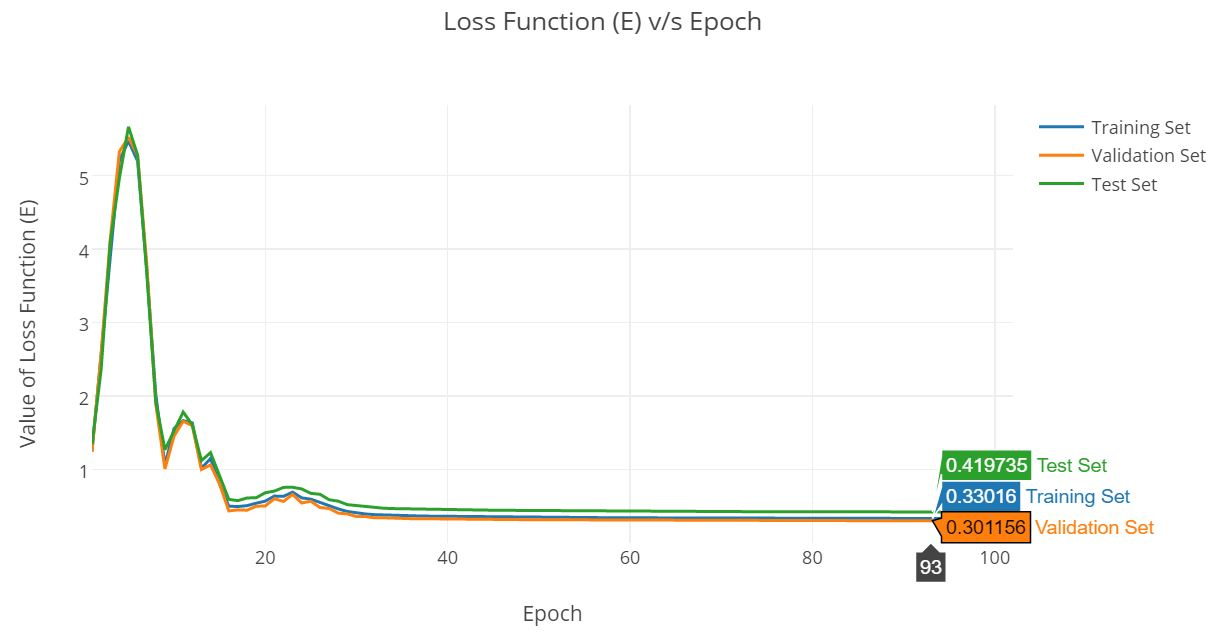
\includegraphics[width=\linewidth]{6b_softmaxLossVsEpoch.JPG}
  \caption{Loss Function(E) v/s Epoch}
  \label{fig:graph 6(b)}
\end{figure}

Graph $\ref{fig:graph 6(b)}$ shows how the training, validation and test errors vary according to the iteration number (epoch) for the same values of hyper-parameters. As evident from the graph, the loss function decreases and stabilizes over time, which corresponds to convergence. As an indicative measure, the values of test, validation and training errors have been displayed for a particular value (93) of epoch.

\subsection{Percent Correct v/s Training Iteration}

The "percent correct" (or accuracy percentage) was plotted over the number of training iterations for the training, hold-out and test sets. 

Parameters used: (same as above)

\begin{figure}
  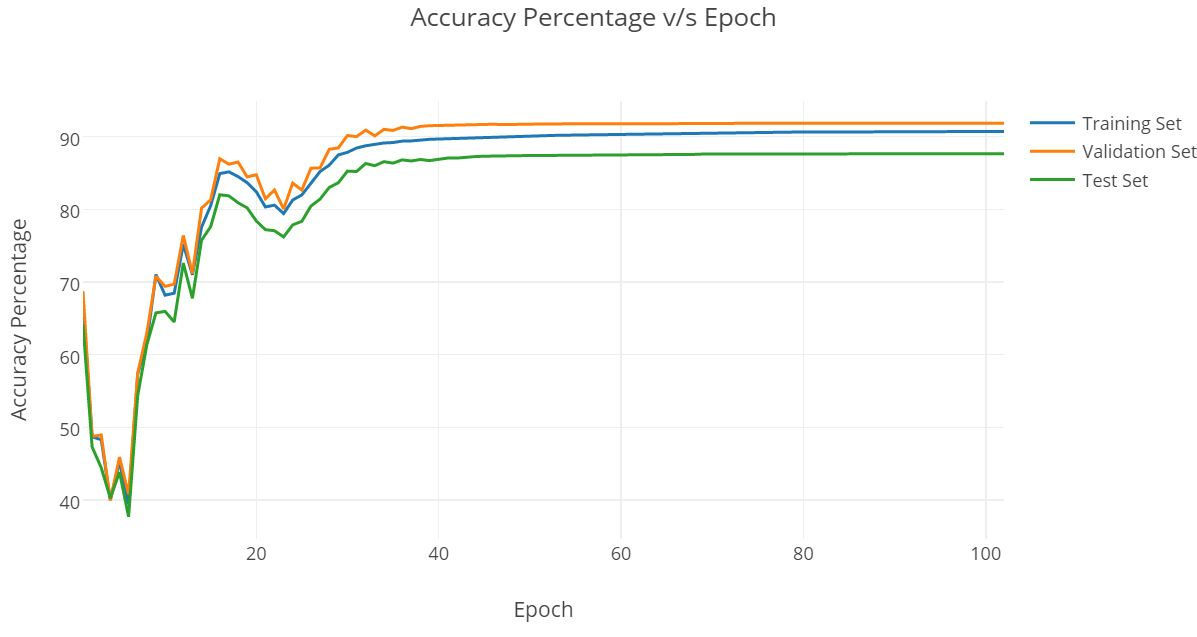
\includegraphics[width=\linewidth]{6c_softmaxAccuracyVsEpoch.JPG}
  \caption{Accuracy Percentage v/s Epoch}
  \label{fig:graph 6(c)}
\end{figure}

Graph \ref{fig:graph 6(c)} shows how the training, validation and test percent correct values vary according to the iteration number (epoch) for the same values of hyper-parameters. As evident from the graph, the accuracy saturates over time and does not improve. The weights learned give the best performance on validation set, followed by training and test set. It is interesting to note that all the values are fairly close to each other and similar in shape, which means that the training set is a good representative of the hold-out and test sets.

\section{Regularization}

\subsection{Update Term Derivations}

Regularization is a commonly used technique to improve the model generalization. We write the regularized loss function \emph{J(w)} as:

$$J(w) = E(w) + \lambda C(w)$$

where \emph{C(w)} is the complexity penalty and $\lambda$ is the strength of regularization. For $\lambda$ = 0, \emph{J} reduces to \emph{E}. Considering $L_{2}$ norm as the complexity penalty, we have:

$$J(w) = E(w) + \lambda ||w||^2$$

To derive the update term, we derive this function with respect to \emph{w}, the weight vector. Hence, we have:

$$\frac{\partial J(w)}{\partial w} = \frac{\partial E(w)}{\partial w} + \lambda\frac{\partial C(w)}{\partial w}$$

We have already calculate the first part of the equation - $\frac{\partial E(w)}{\partial w}$ in Question 1. Hence, according to the question, solving for $\frac{\partial C(w)}{\partial w}$, we have:

$$\frac{\partial C(w)}{\partial w} = \frac{||w||^2}{\partial w} = 2w$$

Therefore, we have:
$$\frac{\partial J(w)}{\partial w} = \frac{\partial E(w)}{\partial w} + 2\lambda w$$

Similarly, for $L_{1}$ norm as the complexity penalty, we have 
$$J(w) = E(w) + \lambda |w|$$
Therefore, 
$$\frac{\partial J(w)}{\partial w} = \frac{\partial E(w)}{\partial w} + \frac{\partial \lambda |w|}{\partial w}$$

$$\frac{\partial J(w)}{\partial w} = \frac{\partial E(w)}{\partial w} + \lambda \frac{\partial |w|}{\partial w}$$

Now, the entry at index \emph{j} of partial derivative of \emph{|w|} can be written as: 

\[
	\frac{\partial |w|}{\partial w_j} = \left\{
                \begin{array}{ll}
                  1, if w_j \geq 0\\
                  -1, otherwise
                \end{array}
              \right.
\]

Thus, the value of $\frac{\partial |w|}{\partial w}$ is A vector of all one's or minues one's depending upon the sign of entries in \emph(w) vector and has the same number of elements as in \emph{w}.

Note that the $L_{1}$ norm is not differentiable at 0. However, all that matters is that we can compute a subgradient / subderivative. Since it's differentiable everywhere else, we can just fill in any "reasonable" value (such as zero) for the gradient at 0.
 
\subsection{Accuracy Percentage v/s Epoch Plot}

The "percent correct" value was plotted over the number of training iterations for the training set, for different lambda values keeping the other hyper-parameters same. 

Parameters used: 

Penalty = $L_{2}$ norm

Learning rate \eta = 0.0001

\begin{figure}
  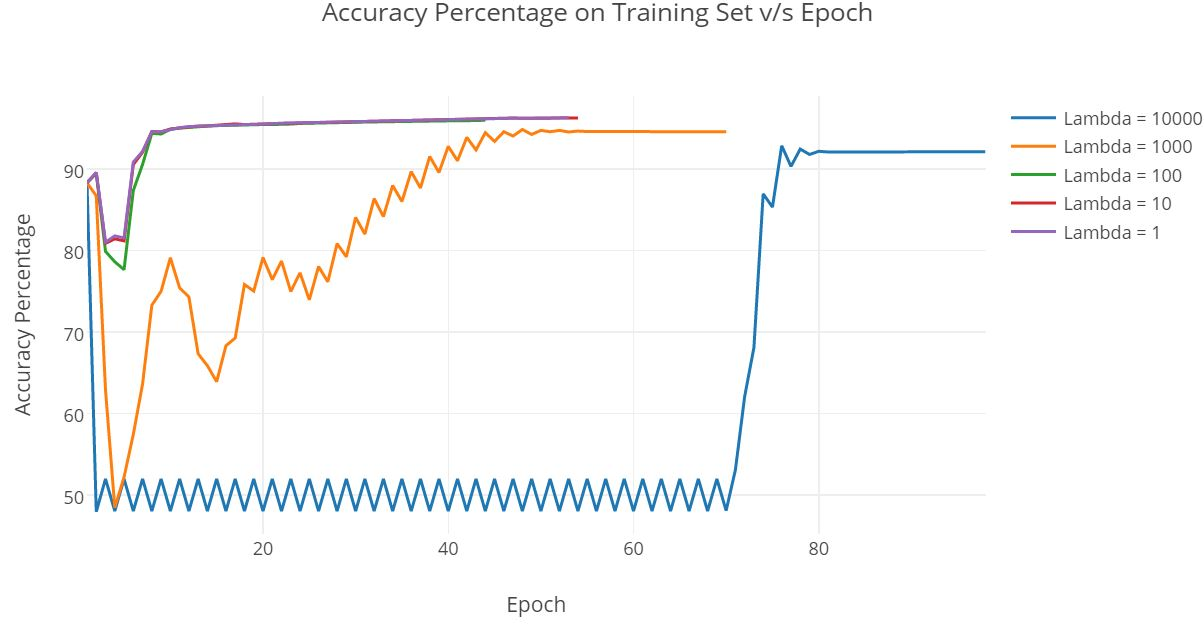
\includegraphics[width=\linewidth]{5_b_negativeInEqn.JPG}
  \caption{Accuracy Percentage v/s Epoch for $L_{2}$ norm}
  \label{fig:graph 5(b) l2}
\end{figure}

Graph \ref{fig:graph 5(b) l2} shows how the accuracy on training data varies according to the iteration number (epoch) for several $\lambda$ values. $\lambda$ is added to avoid over-fitting. Thus, higher the $\lambda$ value, lower will be the accuracy on training set as more emphasis is given to the complexity function rather than the original loss function \emph{E(w)}.

Now for penalty as $L_{1}$ norm and Learning rate $\eta$ = 0.0001, we have:

\begin{figure}
  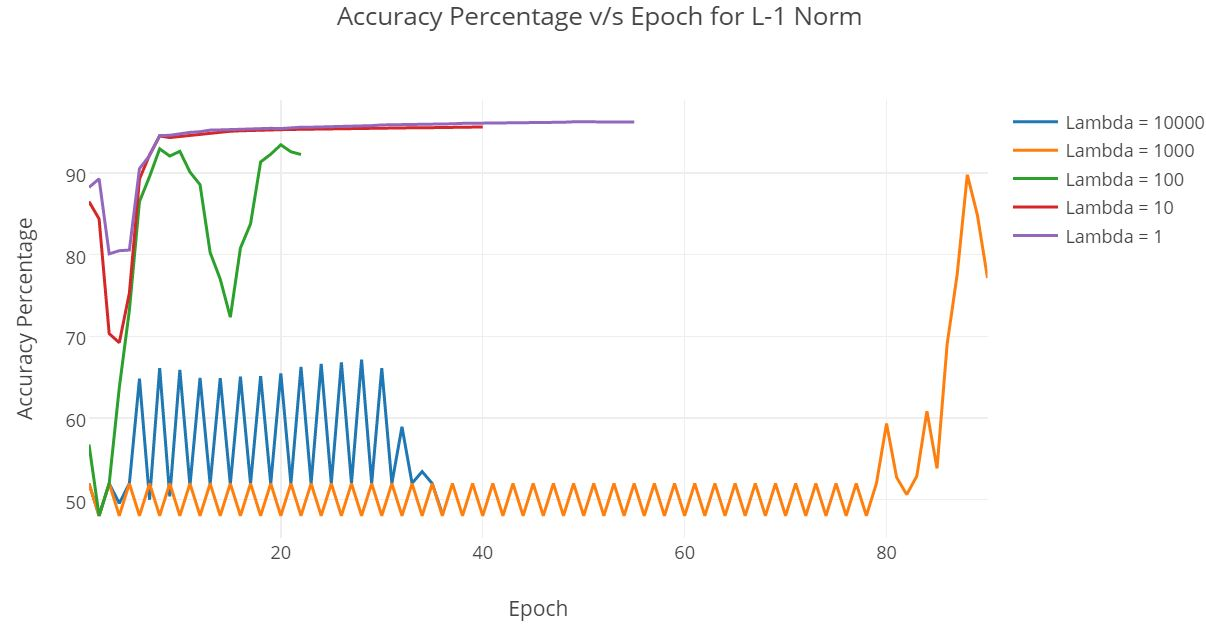
\includegraphics[width=\linewidth]{5_b_L1_new.JPG}
  \caption{Accuracy Percentage v/s Epoch for $L_{1}$ norm}
  \label{fig:graph 5(b) l1}
\end{figure}

Graph \ref{fig:graph 5(b) l1} shows how the accuracy on training data varies according to the iteration number (epoch) for several $\lambda$ values. The same generalization as above holds here as well. Note that the graph line for $\lambda$ = 10000 overlaps with that of $\lambda$ = 1000 and is not visible clearly.

\subsection{Weight Vector Length v/s Training Iteration}

The length of weight vector against training iterations produced a graph as follows for the $L_{2}$ norm case:

\begin{figure}
  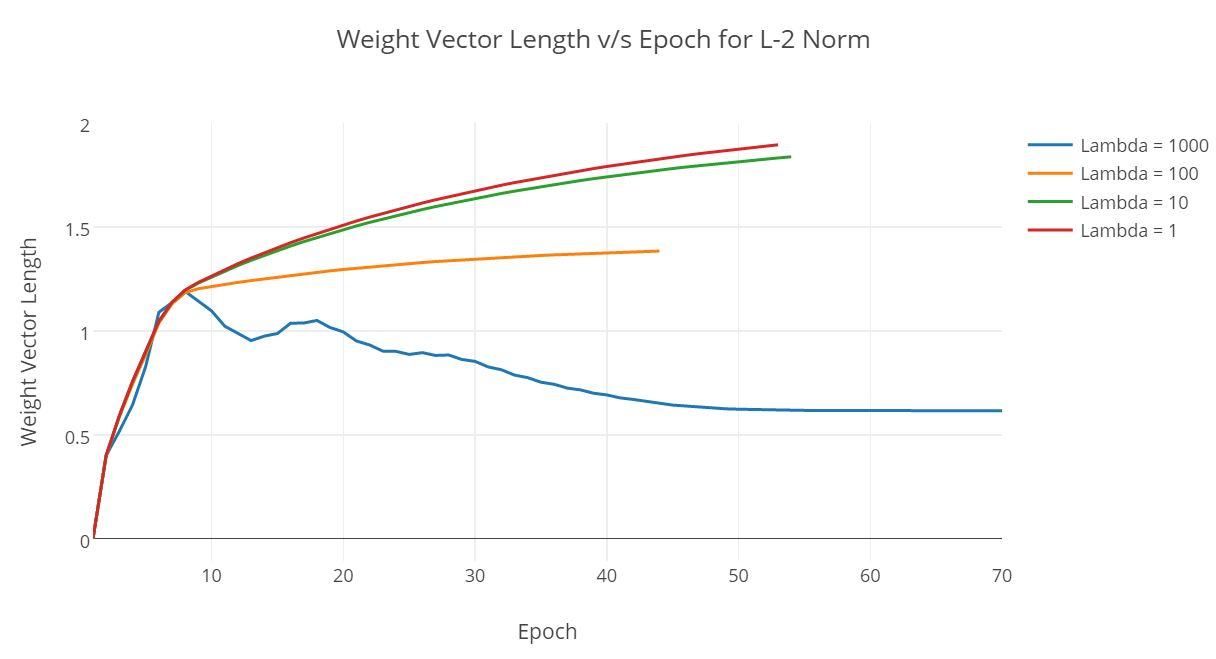
\includegraphics[width=\linewidth]{5_c.JPG}
  \caption{Weight Vector Length v/s Epoch with $L_{2}$ norm}
  \label{fig:graph 5(c) l2}
\end{figure}

For $L_{1}$ norm, it becomes:

\begin{figure}
  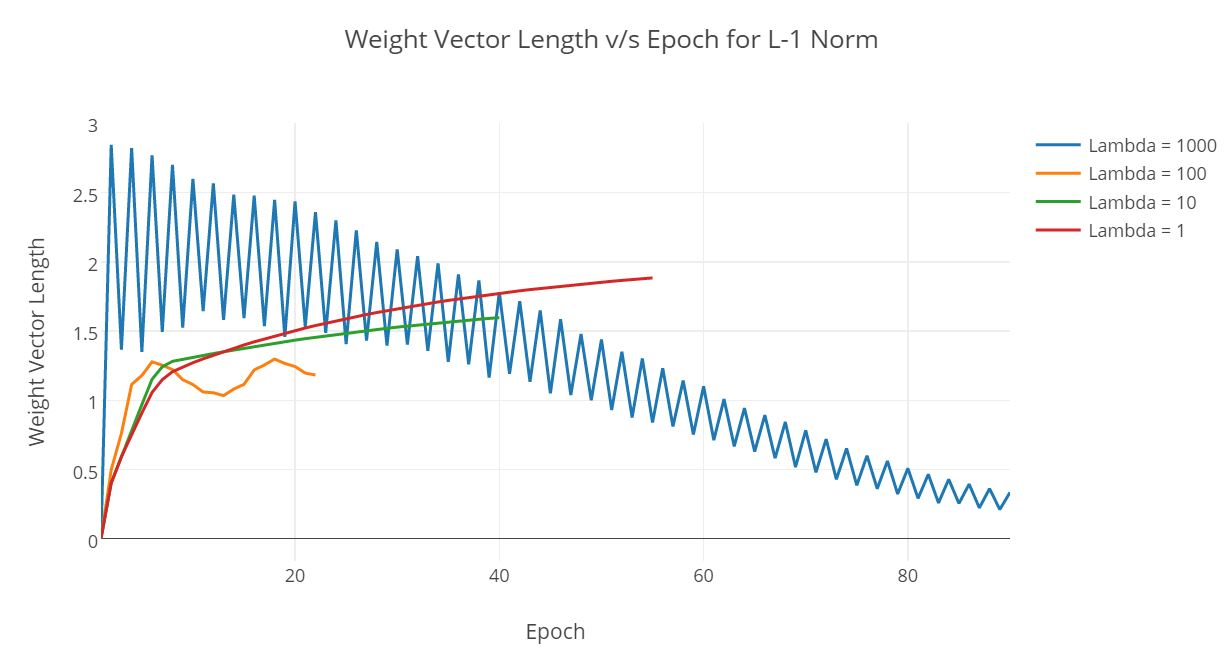
\includegraphics[width=\linewidth]{5_c_negative_l1.JPG}
  \caption{Weight Vector Length v/s Epoch with $L_{1}$ norm}
  \label{fig:graph 5(c) l1}
\end{figure}

Note that the learning rate $\eta$ used was 0.0001 in both the cases.

In both the cases, as $\lambda$ increases, the corresponding weight vector length value decreases. Both these values are inversely related. This is due because as $\lambda$ increases, the overall regularized loss function value tends to increase. However, since our goal is to minimize loss, the weight vector balances this increase in $\lambda$ by decreasing itself. A similar argument is valid for decreasing $\lambda$ values as well.

\subsection{Final Test Error v/s Log(\lambda)}

The plot of final test error for various $\lambda$ values with $L_{2}$ norm penalty is as follows:

\begin{figure}
  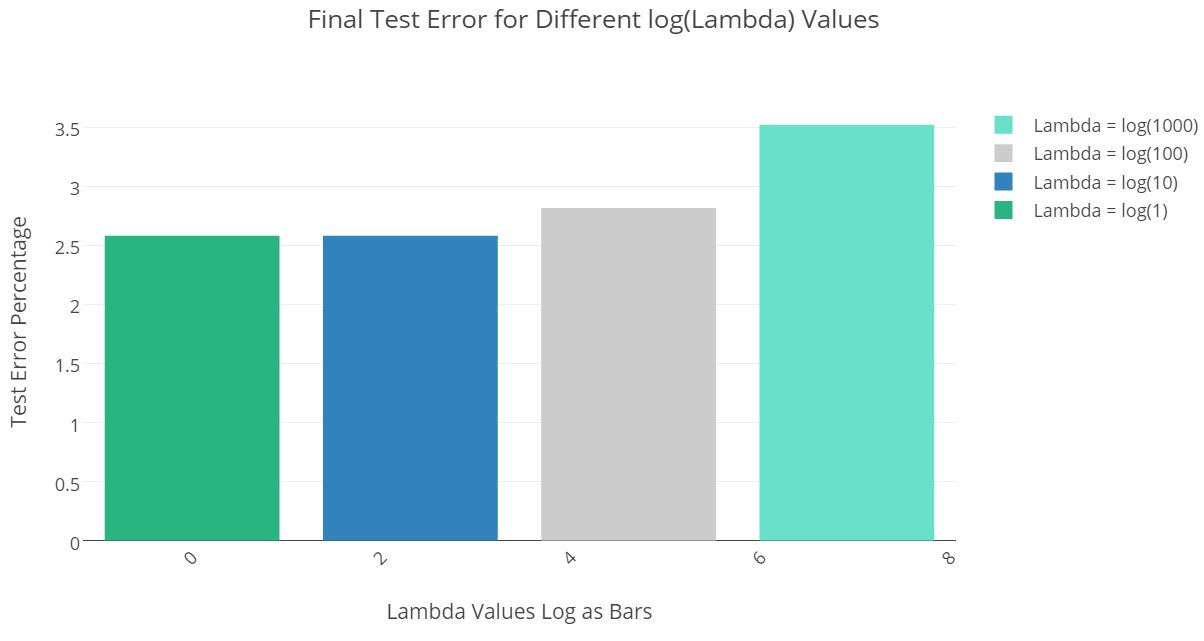
\includegraphics[width=\linewidth]{5_d_negative.JPG}
  \caption{Final Test Error v/s Log(\lambda) $L_{2}$ norm}
  \label{fig:graph 5(d) l2}
\end{figure}

The plot of final test error for various $\lambda$ values with $L_{1}$ norm penalty is as follows:

\begin{figure}
  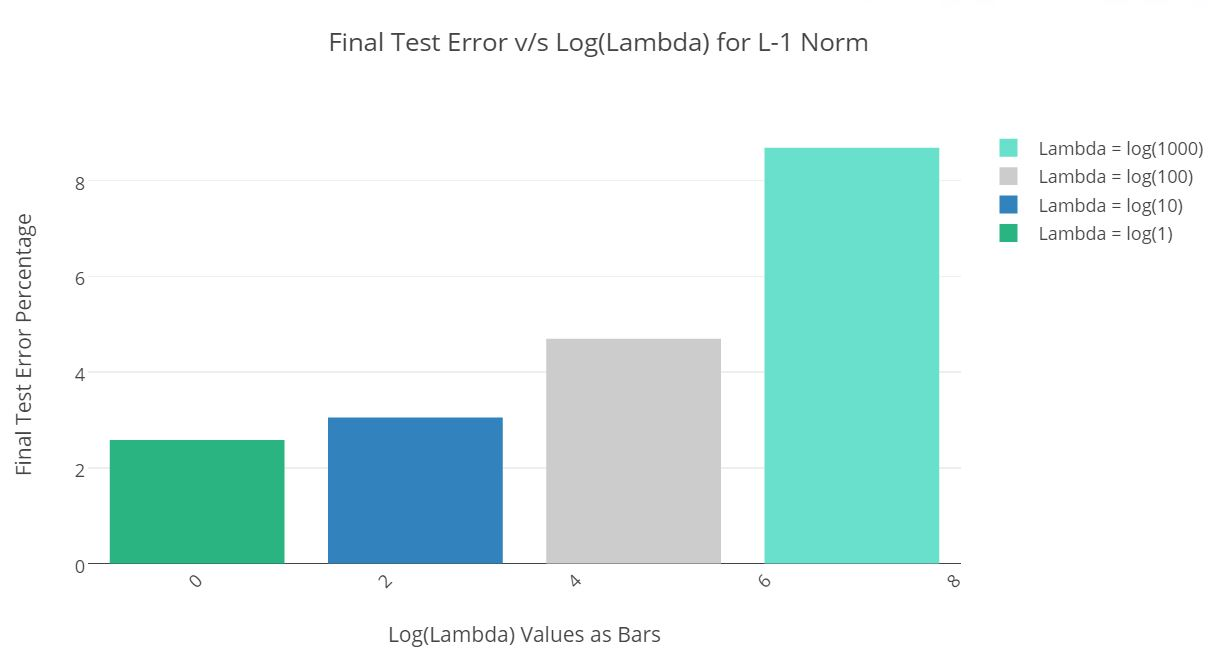
\includegraphics[width=\linewidth]{5_d_l1.JPG}
  \caption{Final Test Error v/s Log(\lambda) $L_{1}$ norm}
  \label{fig:graph 5(d) l1}
\end{figure}

Note that the learning rate $\eta$ used was 0.0001 in both the cases.

In both the above graphs, as $\lambda$ (or log($\lambda$)) increases, the final test error increases. This is because for large $\lambda$ values, the model complexity is low. Beyond a certain level, the complexity may become so low that it no longer fits the data well leading to mis-classification on a large number of points. Increasing $\lambda$ value only decreases the complexity further, leading to even further decline in test accuracy. Similarly, if the $\lambda$ value is too low, the model may become highly complex, so much so that over-fitting happens. Test error in this case will again be large, as the model won't generalize well for points in test set.

\subsection{Weights as Images}

Using learning rate $\eta$ as 0.0001 in both the cases and taking optimum $\lambda$ value 0.0001, the final weight vectors were plotted as images. Here are the findings:

\begin{figure}
  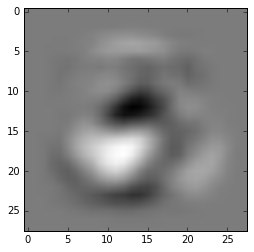
\includegraphics[width=\linewidth]{23WeightsImage_Regularization.PNG}
  \caption{Weight Vector Image for 2's and 3's with $L_{2}$ norm}
  \label{fig:graph 5(e) l2}
\end{figure} 

\begin{figure}
  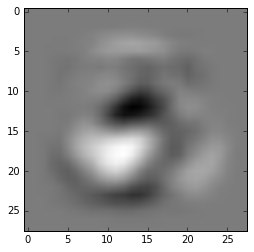
\includegraphics[width=\linewidth]{23Weights_regularization_negative_l1.PNG}
  \caption{Weight Vector Image for 2's and 3's with $L_{1}$ norm}
  \label{fig:graph 5(e) l1}
\end{figure}

\section{Read in Data}

The MNIST data was downloaded from the website at \emph{http://yann.lecun.com/exdb/mnist/} (the same link as given in PA1). To read the data, GitHub library at \emph{https://github.com/akosiorek/CSE/blob/master/MLCV/} was used, which returns the training and testing data in matrix form, and labels as a vectors. Operations were then performed on this data to add a column of ones (bias term) at the beginning and to extract digit specific data (2-3's and 2-8's). Also, the data was restricted to first 20k entries, 10\% of which was allocated to a hold-out set.

\section{Headings: first level}
\label{headings}

All headings should be lower case (except for first word and proper
nouns), flush left, and bold.

First-level headings should be in 12-point type.

\subsection{Headings: second level}

Second-level headings should be in 10-point type.

\subsubsection{Headings: third level}

Third-level headings should be in 10-point type.

\paragraph{Paragraphs}

There is also a \verb+\paragraph+ command available, which sets the
heading in bold, flush left, and inline with the text, with the
heading followed by 1\,em of space.

\section{Citations, figures, tables, references}
\label{others}

These instructions apply to everyone.

\subsection{Citations within the text}

The \verb+natbib+ package will be loaded for you by default.
Citations may be author/year or numeric, as long as you maintain
internal consistency.  As to the format of the references themselves,
any style is acceptable as long as it is used consistently.

The documentation for \verb+natbib+ may be found at
\begin{center}
  \url{http://mirrors.ctan.org/macros/latex/contrib/natbib/natnotes.pdf}
\end{center}
Of note is the command \verb+\citet+, which produces citations
appropriate for use in inline text.  For example,
\begin{verbatim}
   \citet{hasselmo} investigated\dots
\end{verbatim}
produces
\begin{quote}
  Hasselmo, et al.\ (1995) investigated\dots
\end{quote}

If you wish to load the \verb+natbib+ package with options, you may
add the following before loading the \verb+nips_2016+ package:
\begin{verbatim}
   \PassOptionsToPackage{options}{natbib}
\end{verbatim}

If \verb+natbib+ clashes with another package you load, you can add
the optional argument \verb+nonatbib+ when loading the style file:
\begin{verbatim}
   \usepackage[nonatbib]{nips_2016}
\end{verbatim}

As submission is double blind, refer to your own published work in the
third person. That is, use ``In the previous work of Jones et
al.\ [4],'' not ``In our previous work [4].'' If you cite your other
papers that are not widely available (e.g., a journal paper under
review), use anonymous author names in the citation, e.g., an author
of the form ``A.\ Anonymous.''

\subsection{Footnotes}

Footnotes should be used sparingly.  If you do require a footnote,
indicate footnotes with a number\footnote{Sample of the first
  footnote.} in the text. Place the footnotes at the bottom of the
page on which they appear.  Precede the footnote with a horizontal
rule of 2~inches (12~picas).

Note that footnotes are properly typeset \emph{after} punctuation
marks.\footnote{As in this example.}

\subsection{Figures}

All artwork must be neat, clean, and legible. Lines should be dark
enough for purposes of reproduction. The figure number and caption
always appear after the figure. Place one line space before the figure
caption and one line space after the figure. The figure caption should
be lower case (except for first word and proper nouns); figures are
numbered consecutively.

You may use color figures.  However, it is best for the figure
captions and the paper body to be legible if the paper is printed in
either black/white or in color.
\begin{figure}[h]
  \centering
  \fbox{\rule[-.5cm]{0cm}{4cm} \rule[-.5cm]{4cm}{0cm}}
  \caption{Sample figure caption.}
\end{figure}

\subsection{Tables}

All tables must be centered, neat, clean and legible.  The table
number and title always appear before the table.  See
Table~\ref{sample-table}.

Place one line space before the table title, one line space after the
table title, and one line space after the table. The table title must
be lower case (except for first word and proper nouns); tables are
numbered consecutively.

Note that publication-quality tables \emph{do not contain vertical
  rules.} We strongly suggest the use of the \verb+booktabs+ package,
which allows for typesetting high-quality, professional tables:
\begin{center}
  \url{https://www.ctan.org/pkg/booktabs}
\end{center}
This package was used to typeset Table~\ref{sample-table}.

\begin{table}[t]
  \caption{Sample table title}
  \label{sample-table}
  \centering
  \begin{tabular}{lll}
    \toprule
    \multicolumn{2}{c}{Part}                   \\
    \cmidrule{1-2}
    Name     & Description     & Size ($\mu$m) \\
    \midrule
    Dendrite & Input terminal  & $\sim$100     \\
    Axon     & Output terminal & $\sim$10      \\
    Soma     & Cell body       & up to $10^6$  \\
    \bottomrule
  \end{tabular}
\end{table}

\section{Final instructions}

Do not change any aspects of the formatting parameters in the style
files.  In particular, do not modify the width or length of the
rectangle the text should fit into, and do not change font sizes
(except perhaps in the \textbf{References} section; see below). Please
note that pages should be numbered.

\section{Preparing PDF files}

Please prepare submission files with paper size ``US Letter,'' and
not, for example, ``A4.''

Fonts were the main cause of problems in the past years. Your PDF file
must only contain Type 1 or Embedded TrueType fonts. Here are a few
instructions to achieve this.

\begin{itemize}

\item You should directly generate PDF files using \verb+pdflatex+.

\item You can check which fonts a PDF files uses.  In Acrobat Reader,
  select the menu Files$>$Document Properties$>$Fonts and select Show
  All Fonts. You can also use the program \verb+pdffonts+ which comes
  with \verb+xpdf+ and is available out-of-the-box on most Linux
  machines.

\item The IEEE has recommendations for generating PDF files whose
  fonts are also acceptable for NIPS. Please see
  \url{http://www.emfield.org/icuwb2010/downloads/IEEE-PDF-SpecV32.pdf}

\item \verb+xfig+ "patterned" shapes are implemented with bitmap
  fonts.  Use "solid" shapes instead.

\item The \verb+\bbold+ package almost always uses bitmap fonts.  You
  should use the equivalent AMS Fonts:
\begin{verbatim}
   \usepackage{amsfonts}
\end{verbatim}
followed by, e.g., \verb+\mathbb{R}+, \verb+\mathbb{N}+, or
\verb+\mathbb{C}+ for $\mathbb{R}$, $\mathbb{N}$ or $\mathbb{C}$.  You
can also use the following workaround for reals, natural and complex:
\begin{verbatim}
   \newcommand{\RR}{I\!\!R} %real numbers
   \newcommand{\Nat}{I\!\!N} %natural numbers
   \newcommand{\CC}{I\!\!\!\!C} %complex numbers
\end{verbatim}
Note that \verb+amsfonts+ is automatically loaded by the
\verb+amssymb+ package.

\end{itemize}

If your file contains type 3 fonts or non embedded TrueType fonts, we
will ask you to fix it.

\subsection{Margins in \LaTeX{}}

Most of the margin problems come from figures positioned by hand using
\verb+\special+ or other commands. We suggest using the command
\verb+\includegraphics+ from the \verb+graphicx+ package. Always
specify the figure width as a multiple of the line width as in the
example below:
\begin{verbatim}
   \usepackage[pdftex]{graphicx} ...
   \includegraphics[width=0.8\linewidth]{myfile.pdf}
\end{verbatim}
See Section 4.4 in the graphics bundle documentation
(\url{http://mirrors.ctan.org/macros/latex/required/graphics/grfguide.pdf})

A number of width problems arise when \LaTeX{} cannot properly
hyphenate a line. Please give LaTeX hyphenation hints using the
\verb+\-+ command when necessary.

\subsubsection*{Acknowledgments}

Use unnumbered third level headings for the acknowledgments. All
acknowledgments go at the end of the paper. Do not include
acknowledgments in the anonymized submission, only in the final paper.

\section*{References}

References follow the acknowledgments. Use unnumbered first-level
heading for the references. Any choice of citation style is acceptable
as long as you are consistent. It is permissible to reduce the font
size to \verb+small+ (9 point) when listing the references. {\bf
  Remember that you can use a ninth page as long as it contains
  \emph{only} cited references.}
\medskip

\small

[1] Alexander, J.A.\ \& Mozer, M.C.\ (1995) Template-based algorithms
for connectionist rule extraction. In G.\ Tesauro, D.S.\ Touretzky and
T.K.\ Leen (eds.), {\it Advances in Neural Information Processing
  Systems 7}, pp.\ 609--616. Cambridge, MA: MIT Press.

[2] Bower, J.M.\ \& Beeman, D.\ (1995) {\it The Book of GENESIS:
  Exploring Realistic Neural Models with the GEneral NEural SImulation
  System.}  New York: TELOS/Springer--Verlag.

[3] Hasselmo, M.E., Schnell, E.\ \& Barkai, E.\ (1995) Dynamics of
learning and recall at excitatory recurrent synapses and cholinergic
modulation in rat hippocampal region CA3. {\it Journal of
  Neuroscience} {\bf 15}(7):5249-5262.

\end{document}
